% ---
% Chapter 3
% ---
\chapter{A theory for CSP in Coq}
\label{chapter:csp_coq}
% ---

Chapter~\ref{chapter:background} provided an overview of the essential concepts for understanding the implementation of \CSPcoq{}, setting the scene for an in-depth explanation of the language developed in this work. That being said, Chapter~\ref{chapter:csp_coq} explains how we developed a theory for communicating sequential processes in the Coq proof assistant.

Section~\ref{section:syntax} discusses the implementation of the language's abstract and concrete syntaxes, whereas Section~\ref{section:sos} explains how the SOS style of defining language semantics translates into Coq as inductively defined propositions. Afterwards, Section~\ref{section:lts} provides details on both functional and inductive definitions of LTSs, along with further explanation on the GraphViz software integration. Finally, Section~\ref{section:traces} explains how we define traces refinement as an executable property and also presents randomised testing based on this property using the QuickChick tool.

Our Coq characterisation of CSP is structured into the following files. We have a total of 675 LOC (lines of code) of formal definitions, and 94 LOC concerning the definition of special-purpose tactics.

\begin{itemize}
	\item \textbf{syntax.v}: the abstract and concrete syntaxes of \CSPcoq{}.
	\item \textbf{semantics\_sos.v}: the SOS-style semantics of \CSPcoq{}.
	\item \textbf{lts.v} characterisations of LTSs and integration with GraphViz.
	\item \textbf{semantics\_trace.v}: characterisations of traces and integration with QuickChick.
\end{itemize}

We also have 745 LOC of examples illustrating the formalised concepts. All code is available at our GitHub repository: \url{https://github.com/casc2/tg-formal-methods}.

% ---
\section{Syntax}
\label{section:syntax}
% ---

The \CSPcoq{} language provides support to all process constructors and operations discussed in Section~\ref{section:csp}. Those include the processes $ \mathit{\STOP} $ and $ \mathit{\SKIP} $, the operations event prefix, external choice, internal choice, alphabetised parallelism, generalised parallelism, interleaving, sequential composition, and event hiding, in addition to process referencing. This section introduces the reader to the implementation of both abstract and concrete syntaxes of the \CSPcoq{}.

% ---
\subsection{Abstract syntax}
% ---

In order to define these CSP operations in Coq, we declared the following inductive types: \emph{event}, \emph{event\_tau\_tick}, \emph{channel}, \emph{alphabet}, \emph{proc\_body}, and \emph{proc\_def}. The type \emph{event} represents all external events. As we have said before, external events are all events that are neither internal ($ \tau $) nor indicate termination ($ \tick $). The type \emph{event\_tau\_tick} provides not only a constructor for the external events, but also for the especial events $ \tau $ and $ \tick $.

\begin{coqdoccode}
	\coqdocnoindent
	\coqdockw{Definition} \coqdocvar{event} := \coqdocvar{string}.\coqdoceol
	\coqdocnoindent
	\coqdockw{Inductive} \coqdocvar{event\_tau\_tick} :=\coqdoceol
	\coqdocindent{1.00em}
	\ensuremath{|} \coqdocvar{Event} (\coqdocvar{e} : \coqdocvar{event})\coqdoceol
	\coqdocindent{1.00em}
	\ensuremath{|} \coqdocvar{Tau}\coqdoceol
	\coqdocindent{1.00em}
	\ensuremath{|} \coqdocvar{Tick}.\coqdoceol
\end{coqdoccode}

For describing a set of external events, we have the types \emph{channel} and \emph{alphabet}. Apart from considering different names of constructors, they are syntactically equivalent; the difference between these two types being semantic. The type \emph{channel} is used to declare external events that may be communicated in a \CSPcoq{} specification. The constructor provided by the type \emph{alphabet} is applied, for example, to enumerate all external events in the process interface of an alphabetised parallel composition.

\begin{coqdoccode}
	\coqdocnoindent
	\coqdockw{Inductive} \coqdocvar{alphabet} : \coqdockw{Type} :=\coqdoceol
	\coqdocindent{1.00em}
	\ensuremath{|} \coqdocvar{Alphabet} (\coqdocvar{events} : \coqdoctac{set} \coqdocvar{event}).\coqdoceol
	\coqdocnoindent
	\coqdockw{Inductive} \coqdocvar{channel} : \coqdockw{Type} :=\coqdoceol
	\coqdocindent{1.00em}
	\ensuremath{|} \coqdocvar{Channel} (\coqdocvar{events} : \coqdoctac{set} \coqdocvar{event}).\coqdoceol
\end{coqdoccode}

The types \emph{proc\_body} and \emph{proc\_def} define, respectively, constructors for the CSP language (SKIP, STOP, process referencing, event prefix, external choice, internal choice, alphabetised parallelism, generalised parallelism, interleaving, sequential composition, and hiding) and are used to declare new processes (process attribution statement). The constructors made available by \emph{proc\_body} can be combined in order to describe complex behaviour. The type \emph{proc\_def} provides a constructor that makes it possible to identify a process by an identifier, that is, to give it a name.

\begin{coqdoccode}
	\coqdocnoindent
	\coqdockw{Inductive} \coqdocvar{proc\_body} : \coqdockw{Type} :=\coqdoceol
	\coqdocindent{1.00em}
	\ensuremath{|} \coqdocvar{SKIP}\coqdoceol
	\coqdocindent{1.00em}
	\ensuremath{|} \coqdocvar{STOP}\coqdoceol
	\coqdocindent{1.00em}
	\ensuremath{|} \coqdocvar{ProcRef} (\coqdocvar{name} : \coqdocvar{string})\coqdoceol
	\coqdocindent{1.00em}
	\ensuremath{|} \coqdocvar{ProcPrefix} (\coqdocvar{event} : \coqdocvar{event}) (\coqdocvar{proc} : \coqdocvar{proc\_body})\coqdoceol
	\coqdocindent{1.00em}
	\ensuremath{|} \coqdocvar{ProcExtChoice} (\coqdocvar{proc1} \coqdocvar{proc2} : \coqdocvar{proc\_body})\coqdoceol
	\coqdocindent{1.00em}
	\ensuremath{|} \coqdocvar{ProcIntChoice} (\coqdocvar{proc1} \coqdocvar{proc2} : \coqdocvar{proc\_body})\coqdoceol
	\coqdocindent{1.00em}
	\ensuremath{|} \coqdocvar{ProcAlphaParallel} (\coqdocvar{proc1} \coqdocvar{proc2} : \coqdocvar{proc\_body}) (\coqdocvar{alph1} \coqdocvar{alph2} : \coqdocvar{alphabet})\coqdoceol
	\coqdocindent{1.00em}
	\ensuremath{|} \coqdocvar{ProcGenParallel} (\coqdocvar{proc1} \coqdocvar{proc2} : \coqdocvar{proc\_body}) (\coqdocvar{alph} : \coqdocvar{alphabet})\coqdoceol
	\coqdocindent{1.00em}
	\ensuremath{|} \coqdocvar{ProcInterleave} (\coqdocvar{proc1} \coqdocvar{proc2} : \coqdocvar{proc\_body})\coqdoceol
	\coqdocindent{1.00em}
	\ensuremath{|} \coqdocvar{ProcSeqComp} (\coqdocvar{proc1} \coqdocvar{proc2} : \coqdocvar{proc\_body})\coqdoceol
	\coqdocindent{1.00em}
	\ensuremath{|} \coqdocvar{ProcHiding} (\coqdocvar{proc}: \coqdocvar{proc\_body}) (\coqdocvar{alph} : \coqdocvar{alphabet}).\coqdoceol
	\coqdocnoindent
	\coqdockw{Inductive} \coqdocvar{proc\_def} : \coqdockw{Type} :=\coqdoceol
	\coqdocindent{1.00em}
	\ensuremath{|} \coqdocvar{Proc} (\coqdocvar{name} : \coqdocvar{string}) (\coqdocvar{body} : \coqdocvar{proc\_body}).\coqdoceol
\end{coqdoccode}

The last definition of the CSP abstract syntax is \emph{specification}. A CSP specification can be perceived as a file containing multiple channels of events (\emph{ch\_list}) and declarations of processes (\emph{proc\_list}). Ultimately, it is a context that holds information such as all the events that can be performed, and all processes and corresponding definitions that compose a system. The way we introduce this concept in \CSPcoq{} is via a record type. Records are constructions that allow the definition of a set of attributes and propositions, which must be proved to hold when creating an instance of the record.

\begin{coqdoccode}
	\coqdocnoindent
	\coqdockw{Record} \coqdocvar{specification} : \coqdockw{Type} := \coqdocvar{Build\_Spec} \{\coqdoceol
	\coqdocindent{1.00em}
	\coqdocvar{ch\_list} : \coqdocvar{list} \coqdocvar{channel};\coqdoceol
	\coqdocindent{1.00em}
	\coqdocvar{proc\_list} : \coqdocvar{list} \coqdocvar{proc\_def};\coqdoceol
	\coqdocindent{1.00em}
	\coqdocvar{non\_empty\_proc\_ids} : \ensuremath{\lnot} \coqdocvar{In} \coqdocvar{EmptyString} (\coqdocvar{map} \coqdocvar{get\_proc\_id} \coqdocvar{proc\_list});\coqdoceol
	\coqdocindent{1.00em}
	\coqdocvar{non\_empty\_events} : \ensuremath{\lnot} \coqdocvar{In} \coqdocvar{EmptyString} (\coqdocvar{concat\_channels} \coqdocvar{ch\_list});\coqdoceol
	\coqdocindent{1.00em}
	\coqdocvar{no\_dup\_events\_proc\_ids} :
	\coqdoceol
	\coqdocindent{2.00em} \coqdocvar{NoDup} ((\coqdocvar{concat\_channels} \coqdocvar{ch\_list}) ++ (\coqdocvar{map} \coqdocvar{get\_proc\_id} \coqdocvar{proc\_list}));\coqdoceol
	\coqdocindent{1.00em}
	\coqdocvar{no\_missing\_proc\_defs} : \coqdocvar{incl} (\coqdocvar{get\_proc\_refs} \coqdocvar{proc\_list}) (\coqdocvar{map} \coqdocvar{get\_proc\_id} \coqdocvar{proc\_list});\coqdoceol
	\coqdocindent{1.00em}
	\coqdocvar{no\_missing\_events} : \coqdocvar{incl} (\coqdocvar{get\_events} \coqdocvar{proc\_list}) (\coqdocvar{concat\_channels} \coqdocvar{ch\_list})\coqdoceol
	\coqdocnoindent
	\}.\coqdoceol
\end{coqdoccode}

Therefore, when creating a CSP specification in \CSPcoq{}, one needs to prove that the following properties are met. As mentioned in Chapter~\ref{chapter:introduction}, we have developed a special-purpose tactic (\emph{solve\_spec\_ctx\_rules}) that automates the proof of such properties.

\begin{itemize}
	\item The empty string is not a valid identifier for the name of a process\\
	(property: \emph{non\_empty\_proc\_ids}).
	\item The empty string is not a valid identifier for the name of an external event\\
	(property: \emph{non\_empty\_events}).
	\item The name of processes and external events are unique\\
	(property: \emph{no\_dup\_events\_proc\_ids}).
	\item There are no references to undefined processes\\
	(property: \emph{no\_missing\_proc\_defs}).
	\item There are no references to undefined external events\\
	(property: \emph{no\_missing\_events}).
\end{itemize}

To illustrate the \CSPcoq{} abstract syntax, consider the following \CSPM{} processes:
%
\begin{tabbing}
	\hspace*{1em}\= \hspace*{5.4em} \= \kill
	PRINTER := accept -> print -> STOP\\
	MACHINE := TICKET\\
	\>\> [ \{cash, ticket\} || \{cash, change\} ]\\
	\>\> CHANGE
\end{tabbing}
%
\noindent{}and their representations in \CSPcoq{}:
%
\begin{flushleft}
	Proc ``PRINTER'' (ProcPrefix (Event ``accept'') (ProcPrefix (Event ``print'') STOP))
\end{flushleft}

\begin{tabbing}
	\hspace*{1em}\= \hspace*{2em} \= \kill
	Proc ``MACHINE'' (\\
	\>	ProcAlphaParallel (ProcRef ``TICKET'') (ProcRef ``CHANGE'')\\
	\>	(Alphabet (set\_add event\_dec ``cash''\\
	\>\> (set\_add event\_dec ``ticket'' (empty\_set event))))\\
	\>	(Alphabet (set\_add event\_dec ``cash''\\
	\>\> (set\_add event\_dec ``change'' (empty\_set event))))\\
	)
\end{tabbing}

As one can see from the examples above, the abstract syntax -- though it dictates how well-formed expressions are constructed -- is not a pleasant way of writing statements or at least reading them. For that matter, we need a more convenient notation. One that resembles the \CSPM{} operators and, therefore, facilitates both specification and understanding of \CSPcoq{} processes.

% ---
\subsection{Concrete syntax}
\label{sec:concrete-syntax}
% ---

In order to define a more appropriate notation for the \CSPcoq{} language, the command \coqdockw{Notation} was used. It allows the declaration of a new symbolic notation for an existing definition. The examples bellow demonstrate how this command is used to assign symbols (operators) to previously defined constructors.

\begin{coqdoccode}
	\coqdocnoindent
	\coqdockw{Notation} ``a \texttt{-{}-}> P'' := (\coqdocvar{ProcPrefix} \coqdocvar{a} \coqdocvar{P}) (\coqdoctac{at} \coqdockw{level} 80, \coqdoctac{right} \coqdockw{associativity}).\coqdoceol
	\coqdocnoindent
	\coqdockw{Notation} ``P [] Q'' := (\coqdocvar{ProcExtChoice} \coqdocvar{P} \coqdocvar{Q}) (\coqdoctac{at} \coqdockw{level} 90, \coqdoctac{left} \coqdockw{associativity}).\coqdoceol
	\coqdocnoindent
	\coqdockw{Notation} ``P [[ A \symbol{92}\symbol{92} B ]] Q'' := (\coqdocvar{ProcAlphaParallel} \coqdocvar{P} \coqdocvar{Q} (\coqdocvar{Alphabet} \coqdocvar{A}) (\coqdocvar{Alphabet} \coqdocvar{B}))
	\coqdoceol\coqdocnoindent (\coqdoctac{at} \coqdockw{level} 90, \coqdockw{no} \coqdockw{associativity}).\coqdoceol
\end{coqdoccode}

Along with the assignment of a notation symbol, we can specify its \emph{precedence level} and its \emph{associativity}. The precedence level helps Coq parse compound expressions, whereas the associativity setting helps to disambiguate expressions containing multiple occurrences of the same symbol. Coq uses precedence levels from 0 to 100, and left, right, or no associativity.

In the lines above, the prefix operator has the higher precedence among all three operators and has right associativity. Differently, the external choice has left associativity while the alphabetised parallel operator does not associate at all, meaning that parentheses are necessary to create a compound expression with multiple parallel operations. Now, we can use these symbols to rewrite the process examples from the previous section in a much more friendly way.

\begin{tabbing}
	\hspace*{1em}\= \hspace*{6.4em} \= \kill
	``PRINTER'' ::= ``accept'' \texttt{-{}-}> ``print'' \texttt{-{}-}> STOP\\

	``MACHINE'' ::= ProcRef ``TICKET''\\
	\>\> [[ \{\{``cash'', ``ticket''\}\} \textbackslash\textbackslash \ \{\{``cash'', ``change''\}\} ]]\\
	\>\> ProcRef ``CHANGE''
\end{tabbing}

Table~\ref{tab:cspm-csp_coq} displays a comparison between the \CSPM{} operators we have discussed and the \CSPcoq{} language concrete syntax.

\begin{table}[htb]
	\begin{center}
		\caption[The \CSPcoq{} concrete syntax]{The \CSPcoq{} concrete syntax}
		\label{tab:cspm-csp_coq}
		\begin{tabular}{ |l|c|c| }
			\hline
			Constructor & \CSPM{} & \CSPcoq{} \\
			\hline
			Stop & STOP & STOP \\ [0.5ex]
			Skip & SKIP & SKIP \\ [0.5ex]
			Event prefix & e -> P & e -{}-> P \\  [0.5ex]
			External choice & P [] Q & P [] Q \\  [0.5ex]
			Internal choice & P |$ \sim $| Q & P |$ \sim $| Q \\ [0.5ex]
			Alphabetized parallel & P [A || B] Q & P [[A \textbackslash\textbackslash \ B]] Q \\ [0.5ex]
			Generalized parallel & P [| A |] Q & P [| A |] Q \\ [0.5ex]
			Interleave & P ||| Q & P ||| Q \\ [0.5ex]
			Sequential composition & P ; Q & P ;; Q \\ [0.5ex]
			Event hiding & P \textbackslash \ A & P \textbackslash \ A \\ [0.5ex]
			Process definition & P = Q & P ::= Q \\ [0.5ex]
			Process name & P & ProcRef ``P'' \\ [0.5ex]
			\hline
		\end{tabular}
	\end{center}
\end{table}

Apart from some different symbols (necessary to avoid conflicts with reversed keywords -- e.g., ``-{}->'' and ``;;''), and how to refer to other CSP processes (ProRef ``P''), the concrete syntax of \CSPcoq{} is close to that of CSP$_{M}$.

% ---
\section{Structured operational semantics}
\label{section:sos}
% ---

Now that we have a good understanding of how the abstract syntax and also a convenient notation of the \CSPcoq{} language were implemented in Coq, it is time to discuss the language semantics in Coq. All declarations presented in this section are based on the inference rules discussed in Section~\ref{subsection:sos}. More specifically, we will address how those SOS rules were defined in Coq's environment.

Recall the inductive definition of the evenness property exemplified in Section~\ref{section:coq}. In that example, it was possible to rewrite the inference rules for such a property in terms of an inductive declaration in Coq, where each rule was translated into a propositional statement. We will use the same approach to define the semantic rules of \CSPcoq{}.

Initially, a notation was defined to represent the SOS relation, in order to increase the readability of the inductive declaration. Thus, this new notation could be used in the constructors of the relational definition. The following Coq command line,creates the infix notation ``S \# P // a ==> Q'', which can be pronounced ``in the specification \emph{S}, the process \emph{P}, after communicating \emph{a}, behaves like the process \emph{Q}''.

\begin{coqdoccode}
	\coqdocnoindent
	\coqdockw{Reserved Notation} ``S '\#' P '//' a '==>' Q'' (\coqdoctac{at} \coqdockw{level} 150, \coqdoctac{left} \coqdockw{associativity}).\coqdoceol
\end{coqdoccode}

To exemplify the usage of this notation inside our inductive definition, let us revisit the inference rule for the prefix operator. It states that, after performing the event $a$, the process $a \then P$ behaves as $P$.

\begin{prooftree}
	\AxiomC{}
	\UnaryInfC{$ (a \then P) \trans(2)[a] P $}
\end{prooftree}

This structure can be translated into Coq as a single constructor in the SOS relation. Note that this definition relates a specification (\emph{specification}), a behaviour (\emph{proc\_body}), and an event (\emph{event\_tau\_tick}) with another behaviour (\emph{proc\_body}).

\begin{coqdoccode}
	\coqdocnoindent
	\coqdockw{Inductive} \coqdocvar{sosR} : \coqdocvar{specification} \ensuremath{\rightarrow} \coqdocvar{proc\_body} \ensuremath{\rightarrow} \coqdocvar{event\_tau\_tick} \ensuremath{\rightarrow} \coqdocvar{proc\_body} \ensuremath{\rightarrow} \coqdockw{Prop} :=\coqdoceol
	\coqdocindent{1.00em}
	\ensuremath{|} \coqdocvar{prefix\_rule} (\coqdocvar{S} : \coqdocvar{specification}) (\coqdocvar{P} : \coqdocvar{proc\_body}) (\coqdocvar{a} : \coqdocvar{event}) :\coqdoceol
	\coqdocindent{1.50em}
	\coqdocvar{S} \# (\coqdocvar{a} \texttt{-{}-}> \coqdocvar{P}) // \coqdocvar{Event} \coqdocvar{a} ==> \coqdocvar{P}\coqdoceol
\end{coqdoccode}

Considering the defined notation, this constructor can be interpreted as follows: given a specification $ S $, a process $ P $, and an event $ a $, in the context of $ S $, the process \emph{a -{}-> P}, after communicating event $ a $, behaves as the process $ P $. In other words, it is always true that, in the prefix operation $ a \then P $, after $ a $ is performed, it resolves to $ P $.

The constructors \coqdocvar{ext\_choice\_left\_rule} and \coqdocvar{alpha\_parall\_joint\_rule} illustrate part of the formalisation of the external choice and the alphabetised parallelism operations, respectively. Note that each one of these operations need more than one inference rule in order to fully describe their semantics (see Section~\ref{subsection:sos}). The following definitions consider two of these rules.

The \coqdocvar{ext\_choice\_left\_rule} constructor encodes the inference rule that solves the external choice operation for the left operand. As we have explained before, this behaviour is described by the following rule \
%
\begin{prooftree}
	\AxiomC{$ P \trans(2)[a] P' $}
	\RightLabel{\quad ($ a \neq \tau $)}
	\UnaryInfC{$ P \extchoice Q \trans(2)[a] P' $}
\end{prooftree}
%
which translates into the following logical proposition

\begin{coqdoccode}
	\coqdocnoindent
	\ensuremath{|} \coqdocvar{ext\_choice\_left\_rule} (\coqdocvar{S} : \coqdocvar{specification}) (\coqdocvar{P} \coqdocvar{Q} : \coqdocvar{proc\_body}) :\coqdoceol
	\coqdocindent{1.00em}
	\coqdockw{\ensuremath{\forall}} (\coqdocvar{P'} : \coqdocvar{proc\_body}) (\coqdocvar{a} : \coqdocvar{event\_tau\_tick}),\coqdoceol
	\coqdocindent{3.00em}
	\ensuremath{\lnot} \coqdocvar{eq} \coqdocvar{a} \coqdocvar{Tau} \ensuremath{\rightarrow}\coqdoceol
	\coqdocindent{3.00em}
	(\coqdocvar{S} \# \coqdocvar{P} // \coqdocvar{a} ==> \coqdocvar{P'}) \ensuremath{\rightarrow}\coqdoceol
	\coqdocindent{3.00em}
	(\coqdocvar{S} \# \coqdocvar{P} [] \coqdocvar{Q} // \coqdocvar{a} ==> \coqdocvar{P'})
\end{coqdoccode}

In this statement, we can see that the first clause corresponds to the side condition of the inference rule, which guarantees that the event $a$ is not the internal event $ \tau $. The second clause is the main premise of the rule, ensuring that it is possible for the event $ a $ to evolve the process $ P $ into $ P' $ in the specification $ S $. Together, the side condition and the hypothesis establish the necessary conditions to resolve the external choice operation to the left-hand operand.

Similarly, the constructor \coqdocvar{alpha\_parall\_joint\_rule} formalises the inference rule that defines the synchronous communication of an event by two parallel processes (considering alphabetised parallelism). This rule, as we can see from its sequent notation below, has a side condition which guarantees that the event $a$ belongs to the intersection of the processes interfaces. Furthermore, it has two premises, which ensure that this event is able to evolve both operands of the combination, that is, the processes to the left- and to the right-hand side of the parallelism operator can communicate this event.

\begin{prooftree}
	\AxiomC{$ P \trans(2)[a] P' $}
	\AxiomC{$ Q \trans(2)[a] Q' $}
	\RightLabel{\quad ($ a \in A^{\tick} \cap B^{\tick} $)}
	\BinaryInfC{$ P \parallel[A][B] Q \trans(2)[a] P' \parallel[A][B] Q' $}
\end{prooftree}

The side condition and the premises are rewritten in the inductive definition as antecedents of a logical implication.

\begin{coqdoccode}
	\coqdocnoindent
	\ensuremath{|} \coqdocvar{alpha\_parall\_joint\_rule} (\coqdocvar{S} : \coqdocvar{specification}) (\coqdocvar{P} \coqdocvar{Q} : \coqdocvar{proc\_body}) (\coqdocvar{A} \coqdocvar{B} : \coqdoctac{set} \coqdocvar{event}) :\coqdoceol
	\coqdocindent{1.00em}
	\coqdockw{\ensuremath{\forall}} (\coqdocvar{P'} \coqdocvar{Q'} : \coqdocvar{proc\_body}) (\coqdocvar{a} : \coqdocvar{event}),\coqdoceol
	\coqdocindent{3.00em}
	\coqdocvar{set\_In} \coqdocvar{a} (\coqdocvar{set\_inter} \coqdocvar{event\_dec} \coqdocvar{A} \coqdocvar{B}) \ensuremath{\rightarrow}\coqdoceol
	\coqdocindent{3.00em}
	(\coqdocvar{S} \# \coqdocvar{P} // \coqdocvar{Event} \coqdocvar{a} ==> \coqdocvar{P'}) \ensuremath{\rightarrow}\coqdoceol
	\coqdocindent{3.00em}
	(\coqdocvar{S} \# \coqdocvar{Q} // \coqdocvar{Event} \coqdocvar{a} ==> \coqdocvar{Q'}) \ensuremath{\rightarrow}\coqdoceol
	\coqdocindent{3.00em}
	\coqdocvar{S} \# \coqdocvar{P} [[ \coqdocvar{A} \symbol{92}\symbol{92} \coqdocvar{B} ]] \coqdocvar{Q} // \coqdocvar{Event} \coqdocvar{a} ==> \coqdocvar{P'} [[ \coqdocvar{A} \symbol{92}\symbol{92} \coqdocvar{B} ]] \coqdocvar{Q'}\coqdoceol
\end{coqdoccode}

Note that this constructor does not consider the $ \tick $ event as a possible synchronisation event, even though it is included in the inference rule (side condition) we saw above. In Coq, external events and $\tick$ are defined using different constructors (\emph{Event} and \emph{Tick}), and, thus, cannot be part of the same set. We need to create different rules for each one. Therefore, the constructor \coqdocvar{alpha\_parall\_tick\_joint\_rule} formalises this joint step when the performed event is $\tick$. The term \emph{event\_dec} provides evidence that the comparison of events is decidable.

The last example of constructor we want to highlight from the inductive definition of the SOS is the \emph{process reference} operation. This constructor defines the rule for unfolding a process definition inside the body of another process.

\begin{coqdoccode}
	\coqdocnoindent
	\ensuremath{|} \coqdocvar{reference\_rule} (\coqdocvar{S} : \coqdocvar{specification}) (\coqdocvar{P} : \coqdocvar{proc\_body}) (\coqdocvar{name} : \coqdocvar{string}) :\coqdoceol
	\coqdocindent{1.00em}
	\coqdockw{\ensuremath{\forall}} (\coqdocvar{Q} : \coqdocvar{proc\_body}),\coqdoceol
	\coqdocindent{3.00em}
	\coqdocvar{eq} \coqdocvar{P} (\coqdocvar{ProcRef} \coqdocvar{name}) \ensuremath{\rightarrow}\coqdoceol
	\coqdocindent{3.00em}
	\coqdocvar{eq} (\coqdocvar{get\_proc\_body} \coqdocvar{S} \coqdocvar{name}) (\coqdocvar{Some} \coqdocvar{Q}) \ensuremath{\rightarrow}\coqdoceol
	\coqdocindent{3.00em}
	\coqdocvar{S} \# \coqdocvar{P} // \coqdocvar{Tau} ==> \coqdocvar{Q}\coqdoceol
\end{coqdoccode}

As we can see, there are two premises for successfully unfolding a definition. First, $P$ must be of the form \coqdocvar{ProcRef} \coqdocvar{name}, where \coqdocvar{ProcRef} is a constructor of type \coqdocvar{proc\_body}, and \coqdocvar{name} is a string that identifies a process. Second, the process referenced by \coqdocvar{ProcRef} \coqdocvar{name} must be defined in the specification. The auxiliary function \coqdocvar{get\_proc\_body} searches for this definition inside the specification, while the equality ensures that this search results in ``$ Some \ Q $'', where $ Q $ is a process body. If such a process name is not found in the specification, this auxiliary function yields ``\emph{None}''.

Although we reflect the original reference rule, it is important to emphasise that our definition in Coq differs from the one implemented by the FDR tool. As explained in~\citeonline[p.~203, footnote 7]{roscoe:ucs}, it does not introduce this $\tau$ action to prevent from increasing the size of the state space. However, as a consequence, FDR diverges (stops responding) when analysing definitions such as $P = P$. This does not happen in \CSPcoq{}.

% ---
\section{Labelled transition systems}
\label{section:lts}
% ---

Now, considering the SOS presented before and implemented in Coq, we discuss another way of representing processes, based on the idea of labelled transition systems (LTSs). This section will cover how the LTS concept is embedded in Coq via functional and inductive definitions, and how \CSPcoq{} provides support to the GraphViz software, which enables a graphical visualisation of CSP processes.

A labelled transition system consists of a non-empty set of states $ S $, with a designated initial state $ P_{0} $, a set of labels $ L $, and a ternary relation (a set of triples of the form $(P,x,Q)$, meaning that the state $ P $ can perform an action labelled as $ x $ and move to state $ Q $). In Coq, we define an LTS in two different and complementary ways: a computable function and a relation.

To illustrate these definitions, consider the following \CSPcoq{} specification.

\begin{coqdoccode}
	\coqdocnoindent
	\coqdockw{Definition} \coqdocvar{SPEC} : \coqdocvar{specification}.\coqdoceol
	\coqdocnoindent
	\coqdockw{Proof}.\coqdoceol
	\coqdocindent{1.00em}
	\coqdocvar{solve\_spec\_ctx\_rules} (\coqdoceol
	\coqdocindent{2.00em}
	\coqdocvar{Build\_Spec}\coqdoceol
	\coqdocindent{2.00em}
	[ \coqdocvar{Channel} \{\{``a'', ``b'', ``c''\}\} ]\coqdoceol
	\coqdocindent{2.00em}
	[ ``P'' ::= (``a'' -{}-> ``b'' -{}-> \coqdocvar{STOP}) [] (``c'' -{}-> \coqdocvar{STOP}) ]\coqdoceol
	\coqdocindent{1.00em}
	).\coqdoceol
	\coqdocnoindent
	\coqdockw{Defined}.\coqdoceol
\end{coqdoccode}

Initially, the process ``P'' can perform either ``a'' or ``c''. If ``a'' gets communicated, the external choice resolves to the process ``b'' -{}-> STOP, which can then perform ``b'' and finish the execution. Differently, if the event ``c'' gets communicated instead, then the composition resolves to the process STOP and also terminates. Therefore, we can list three transitions for ``P'': from state \emph{(``a'' -{}-> ``b'' -{}-> STOP) [] (``c'' -{}-> STOP)} to state \emph{``b'' -{}-> STOP} by performing ``a'', from state \emph{(``a'' -{}-> ``b'' -{}-> STOP) [] (``c'' -{}-> STOP)} to state STOP by performing \emph{``c''}, and from state \emph{``b'' -{}-> STOP} to state \emph{STOP} by performing ``b''. To better describe these transitions, we will use the 3-tuple notation ($ P $, $ a $, $ Q $), where $ P $ is the source state, $ a $ is the action (event), and $ Q $ is the target state.

We can apply the same intuition from this example in the implementation of a functional definition of LTSs in Coq. Starting from the initial state $S_{0}$, compute all the immediate transitions available from this state, that is, all 3-tuples where the target states can be reached in one step from $ S_{0} $. Mark the initial state as ``visited'' and mark any other state discovered in the previous step as ``not visited''. Then, repeat this step for each unvisited state until there are no states to be visited anymore.

Let \coqdocvar{compute\_ltsR} be the function that implements the idea described in the previous paragraph, the following Coq command computes the set of transitions of ``P''. We omit here the formal definition of this function, but it is available at our GitHub repository.

\begin{coqdoccode}
	\coqdocnoindent
	\coqdockw{Compute} \coqdocvar{compute\_ltsR} \coqdocvar{SPEC} ``P'' 1000.\coqdoceol
\end{coqdoccode}

\begin{tabbing}
	\hspace*{2.5em}\= \hspace*{2em} \= \kill
	= Some\\
	\>	[(``a'' -{}-> ``b'' -{}-> STOP [] ``c'' -{}-> STOP, Event ``a'', ``b'' -{}-> STOP);\\
	\>	(``a'' -{}-> ``b'' -{}-> STOP [] ``c'' -{}-> STOP, Event ``c'', STOP);\\
	\>	(``b'' -{}-> STOP, Event ``b'', STOP)]\\
	: option (set transition)
\end{tabbing}

Note that we need to provide a natural number to the function \coqdocvar{compute\_ltsR} (e.g., 1000). In Coq, to ensure termination, every recursive definition (\coqdockw{Fixpoint}) should have an argument that explicitly decreases in each recursive call. During recursion, since new states may be reached, Coq cannot automatically infer what is the decreasing argument. The natural number ensures this premise (decreasing argument). Therefore, the number of recursive calls is limited by the provided number. However, it is also important to emphasise that, from the yielded result, one can easily assess whether the transition relation has been fully constructed. If the provided argument is not enough for computing all transitions, the function yields \emph{None} instead of \emph{Some} list.

We can prove the correctness of our functional definition for computing LTSs by means of the SOS presented in Section~\ref{section:sos}. If $ T $ is the set of transitions in the LTS representation of process $ P $, then every possible communication of $ P $ -- and its components (inner processes) -- is present in $ T $, and every transition in $ T $ is a valid communication of process $ P $ (or the sub-processes that make up $ P $). With this in mind, we provide an inductive definition for LTSs, which is based on the underlying SOS. Nevertheless, the prove of correctness of \coqdocvar{compute\_ltsR} is left as future work.

Given a specification ($S$), a process identifier ($name$), and a set of transitions ($T$), the propositional function \emph{ltsR} yields a predicate that is true if $T$ is the set of transitions of $P$, according to the \CSPcoq{} SOS. First, $name$ needs to be a process defined in the specification, and $T$ may not have duplicate entries. If these two conditions hold, we say that $T$ is the correct of transitions if it is related to the definition of $P$ (i.e., its \emph{body}) by the inductively defined proposition \emph{ltsR'}.

\begin{coqdoccode}
	\coqdocnoindent
	\coqdockw{Definition} \coqdocvar{ltsR} (\coqdocvar{S} : \coqdocvar{specification}) (\coqdocvar{name} : \coqdocvar{string}) (\coqdocvar{T} : \coqdoctac{set} \coqdocvar{transition}) : \coqdockw{Prop} :=\coqdoceol
	\coqdocindent{1.00em}
	\coqdockw{match} \coqdocvar{get\_proc\_body} \coqdocvar{S} \coqdocvar{name} \coqdockw{with}\coqdoceol
	\coqdocindent{1.00em}
	\ensuremath{|} \coqdocvar{Some} \coqdocvar{body} \ensuremath{\Rightarrow} \coqdocvar{NoDup} \coqdocvar{T} \ensuremath{\land} \coqdocvar{ltsR'} \coqdocvar{S} \coqdocvar{T} [\coqdocvar{body}] \coqdocvar{nil}\coqdoceol
	\coqdocindent{1.00em}
	\ensuremath{|} \coqdocvar{None} \ensuremath{\Rightarrow} \coqdocvar{False}\coqdoceol
	\coqdocindent{1.00em}
	\coqdockw{end}.\coqdoceol
\end{coqdoccode}

The inductively defined proposition (LTS relation) is formalised as follows \emph{ltsR'}. It has two constructors, which capture (inductively) a breadth-first search. Its last two arguments (\coqdoctac{set} \coqdocvar{proc\_body}) control the visited and the to-visit states (represented as process behaviours), respectively. The first constructor (\coqdocvar{lts\_empty\_rule}) states that when no states remain to be visited (\emph{nil}), the corresponding LTS is empty (\emph{nil}).

\begin{coqdoccode}
	\coqdocnoindent
	\coqdockw{Inductive} \coqdocvar{ltsR'} :\coqdoceol
	\coqdocindent{1.00em}
	\coqdocvar{specification} \ensuremath{\rightarrow} \coqdoceol
	\coqdocindent{1.00em}
	\coqdoctac{set} \coqdocvar{transition} \ensuremath{\rightarrow} \coqdoceol
	\coqdocindent{1.00em}
	\coqdoctac{set} \coqdocvar{proc\_body} \ensuremath{\rightarrow} \coqdoceol
	\coqdocindent{1.00em}
	\coqdoctac{set} \coqdocvar{proc\_body} \ensuremath{\rightarrow} \coqdoceol
	\coqdocindent{1.00em}
	\coqdockw{Prop} :=\coqdoceol
	\coqdocindent{1.00em}
	\ensuremath{|} \coqdocvar{lts\_empty\_rule} (\coqdocvar{S} : \coqdocvar{specification}) (\coqdocvar{visited} : \coqdoctac{set} \coqdocvar{proc\_body}) :\coqdoceol
	\coqdocindent{3.00em}
	\coqdocvar{ltsR'} \coqdocvar{S} \coqdocvar{nil} \coqdocvar{nil} \coqdocvar{visited}\coqdoceol
	\coqdocindent{1.00em}
\end{coqdoccode}

The second constructor (\coqdocvar{lts\_inductive\_rule}) captures the induction step of our definition. Provided that:
%
\begin{itemize}
	\item $P$ is an arbitrary state/process;
	\item $T$ is a set of transitions;
	\item $T'$ is the set of transitions emanating from $P$ in $T$, such that a triple $(P,a,P')$ is in $T'$ if, and only if, according to the SOS, $P$ behaves as $P'$ after performing $a$;
	\item $T''$ is defined as $T - T'$ (i.e., the transitions not emanating from $P$ in $T$)
\end{itemize}
%
we can prove that $T$ is the set of transitions of $P :: tl$ (i.e., the process $P$ follower by an arbitrary list of other states/processes still to be visited -- the tail \emph{tl}), if we prove that $T''$ is the set of transitions of \emph{to\_visit}, which is the list of states to visit updated by including the states reached by $T'$ and excluding the already visited ones (\emph{visited'}), which includes the previously visited states in addition to $P$.

\begin{coqdoccode}
	\ensuremath{|} \coqdocvar{lts\_inductive\_rule}\coqdoceol
	\coqdocindent{4.00em}
	(\coqdocvar{S} : \coqdocvar{specification})\coqdoceol
	\coqdocindent{4.00em}
	(\coqdocvar{T} : \coqdoctac{set} \coqdocvar{transition})\coqdoceol
	\coqdocindent{4.00em}
	(\coqdocvar{P} : \coqdocvar{proc\_body})\coqdoceol
	\coqdocindent{4.00em}
	(\coqdocvar{tl} \coqdocvar{visited} : \coqdoctac{set} \coqdocvar{proc\_body}) :\coqdoceol
	\coqdocindent{3.00em}
	\coqdockw{let} \coqdocvar{T'} := \coqdocvar{transitions\_from} \coqdocvar{P} \coqdocvar{T} \coqdoctac{in}\coqdoceol
	\coqdocindent{3.00em}
	\coqdockw{let} \coqdocvar{T'{}'} := \coqdocvar{set\_diff} \coqdocvar{transition\_eq\_dec} \coqdocvar{T} \coqdocvar{T'} \coqdoctac{in}\coqdoceol
	\coqdocindent{3.00em}
	\coqdockw{let} \coqdocvar{visited'} := \coqdocvar{set\_add} \coqdocvar{proc\_body\_eq\_dec} \coqdocvar{P} \coqdocvar{visited} \coqdoctac{in}\coqdoceol
	\coqdocindent{3.00em}
	\coqdockw{let} \coqdocvar{to\_visit} := \coqdocvar{set\_diff} \coqdocvar{proc\_body\_eq\_dec}\coqdoceol
	\coqdocindent{12.00em}
	(\coqdocvar{set\_union} \coqdocvar{proc\_body\_eq\_dec} \coqdocvar{tl} (\coqdocvar{target\_proc\_bodies} \coqdocvar{T'}))\coqdoceol
	\coqdocindent{12.00em}
	\coqdocvar{visited'} \coqdoctac{in}\coqdoceol
	\coqdocindent{3.00em}
	(\coqdockw{\ensuremath{\forall}} (\coqdocvar{a} : \coqdocvar{event\_tau\_tick}) (\coqdocvar{P'} : \coqdocvar{proc\_body}),\coqdoceol
	\coqdocindent{4.50em}
	(\coqdocvar{S} \# \coqdocvar{P} // \coqdocvar{a} ==> \coqdocvar{P'}) \ensuremath{\leftrightarrow} \coqdocvar{In} (\coqdocvar{P},\coqdocvar{a},\coqdocvar{P'}) \coqdocvar{T'}) \ensuremath{\rightarrow}\coqdoceol
	\coqdocindent{3.00em}
	\coqdocvar{ltsR'} \coqdocvar{S} \coqdocvar{T'{}'} \coqdocvar{to\_visit} \coqdocvar{visited'} \ensuremath{\rightarrow}\coqdoceol
	\coqdocindent{3.00em}
	\coqdocvar{ltsR'} \coqdocvar{S} \coqdocvar{T} (\coqdocvar{P} :: \coqdocvar{tl}) \coqdocvar{visited}.\coqdoceol
\end{coqdoccode}

The successive application of the induction step will progressively relate a set of transitions with all states reached from the initial one. This formal definition can be used to prove that a particular result of \coqdocvar{compute\_ltsR} is correct, as illustrated in the following example, where $ls$ is the list yielded by \coqdocvar{compute\_ltsR} \coqdocvar{SPEC} ``P'' 1000.

\begin{coqdoccode}
	\coqdocnoindent
	\coqdockw{Example} \coqdocvar{lts1\_is\_valid} :\coqdoceol
	\coqdocindent{1.00em}
	\coqdocvar{ltsR} \coqdocvar{SPEC} ``P'' ls.\coqdoceol
	\coqdocnoindent
	\coqdockw{Proof}. $\ldots$ \coqdockw{Qed.}\coqdoceol
\end{coqdoccode}

During the development of this work, we have used this idea to validate the function \coqdocvar{compute\_ltsR}; proving that the computed LTSs are correct indeed.

% ---
\subsection{GraphViz integration}
% ---

GraphViz is an open source graph visualisation software that takes descriptions of graphs in simple textual languages -- in our case, the DOT language -- and creates diagrams in useful formats, such as SVG and PDF. Moreover, this tool allows the customisation of these diagrams, modifying colors, fonts, hyperlinks, and using custom node shapes. Providing support for this software enables \CSPcoq{} users to generate a graph from the description of an LTS with one command line. That way, the behaviour of a process may be inspected and validated more easily, since a visual representation is available.

In order to build the description of a graph in the DOT language, it is necessary to define a mapping of the constructors of the types \coqdocvar{event\_tau\_tick} and \coqdocvar{proc\_body} to the \coqdocvar{string} type. That way, it is possible to convert each tuple from the LTS into a statement that corresponds to a transition of a graph in the DOT syntax. One way to achieve this in Coq is through the \coqdockw{Coercion} command, which assigns a conversion function that maps an expression of one type into another. For example, consider the following coercion from the type \coqdocvar{event\_tau\_tick} to the type \coqdocvar{string}.

\begin{coqdoccode}
	\coqdocnoindent
	\coqdockw{Definition} \coqdocvar{event\_tau\_tick\_to\_str} (\coqdocvar{e} : \coqdocvar{event\_tau\_tick}) : \coqdocvar{string} :=\coqdoceol
	\coqdocindent{1.00em}
	\coqdockw{match} \coqdocvar{e} \coqdockw{with}\coqdoceol
	\coqdocindent{1.00em}
	\ensuremath{|} \coqdocvar{Tau} \ensuremath{\Rightarrow} ``$ \tau $''\coqdoceol
	\coqdocindent{1.00em}
	\ensuremath{|} \coqdocvar{Tick} \ensuremath{\Rightarrow} ``$ \tick $''\coqdoceol
	\coqdocindent{1.00em}
	\ensuremath{|} \coqdocvar{Event} \coqdocvar{a} \ensuremath{\Rightarrow} \coqdocvar{a}\coqdoceol
	\coqdocindent{1.00em}
	\coqdockw{end}.\coqdoceol
	\coqdocemptyline
	\coqdocnoindent
	\coqdockw{Coercion} \coqdocvar{event\_tau\_tick\_to\_str} : \coqdocvar{event\_tau\_tick} >-> \coqdocvar{string}.\coqdoceol
\end{coqdoccode}

As we can see from the code snippet above, initially, we defined a function that takes an element of type \coqdocvar{event\_tau\_tick} and yields a string representation of this element. Then, a coercion between the two types is established: from this point on, Coq will convert an element of type \coqdocvar{event\_tau\_tick} into a string whenever it is necessary.

Once the possible coercions are stated, we define in Coq the function \coqdocvar{generate\_dot} to create the description of a graph in the DOT language from the set of tuples that make up the LTS. The intuition behind this function is as follows. The first tuple to be processed has its starting state identified as the graph's initial node (bold and red border), and each tuple -- the first included -- is rewritten as a DOT syntax transition statement. In other words, the tuple $(P, e, Q)$ is translated to the string ``<P> -> <Q> [label = <e>];'' by this function, as shown in the definitions below. Note that the function \coqdocvar{generate\_dot} relies on the auxiliary and recursive function \coqdocvar{generate\_dot'}.

\begin{coqdoccode}
	\coqdocnoindent
	\coqdockw{Fixpoint} \coqdocvar{generate\_dot'} (\coqdocvar{lts} : \coqdoctac{set} \coqdocvar{transition}) : \coqdocvar{string} :=\coqdoceol
	\coqdocindent{1.00em}
	\coqdockw{match} \coqdocvar{lts} \coqdockw{with}\coqdoceol
	\coqdocindent{1.00em}
	\ensuremath{|} \coqdocvar{nil} \ensuremath{\Rightarrow} ``''\coqdoceol
	\coqdocindent{1.00em}
	\ensuremath{|} (\coqdocvar{P}, \coqdocvar{e}, \coqdocvar{Q}) :: \coqdocvar{tl} \ensuremath{\Rightarrow} `` <'' ++ \coqdocvar{P} ++ ``> -> <'' ++ \coqdocvar{Q} ++ ``>'' ++\coqdoceol
	\coqdocindent{9.30em}`` [label=<'' ++ \coqdocvar{e} ++ ``>];'' ++ (\coqdocvar{generate\_dot'} \coqdocvar{tl})\coqdoceol
	\coqdocindent{1.00em}
	\coqdockw{end}.\coqdoceol
	\coqdocemptyline
	\coqdocnoindent
	\coqdockw{Definition} \coqdocvar{style\_initial\_state} (\coqdocvar{P} : \coqdocvar{proc\_body}) : \coqdocvar{string} :=\coqdoceol
	\coqdocindent{1.00em} ``<'' ++ \coqdocvar{P} ++ ``> [style=bold, color=red];''.\coqdoceol
	\coqdocemptyline
	\coqdocnoindent
	\coqdockw{Definition} \coqdocvar{generate\_dot} (\coqdocvar{lts} : \coqdocvar{option} (\coqdoctac{set} \coqdocvar{transition})) : \coqdocvar{string} :=\coqdoceol
	\coqdocindent{1.00em}
	\coqdockw{match} \coqdocvar{lts} \coqdockw{with}\coqdoceol
	\coqdocindent{1.00em}
	\ensuremath{|} \coqdocvar{Some} ((\coqdocvar{P}, \coqdocvar{e}, \coqdocvar{Q}) :: \coqdocvar{tl}) \ensuremath{\Rightarrow}\coqdoceol
	\coqdocindent{2.00em}
	``digraph LTS \{ '' ++ (\coqdocvar{style\_initial\_state} \coqdocvar{P}) ++\coqdoceol
	\coqdocindent{2.00em} (\coqdocvar{generate\_dot'} ((\coqdocvar{P}, \coqdocvar{e}, \coqdocvar{Q}) :: \coqdocvar{tl})) ++ `` \}''\coqdoceol
	\coqdocindent{1.00em}
	\ensuremath{|} \coqdocvar{\_} \ensuremath{\Rightarrow} ``''\coqdoceol
	\coqdocindent{1.00em}
	\coqdockw{end}.\coqdoceol
\end{coqdoccode}

To demonstrate these definitions, recall the MACHINE example from Section~\ref{sec:concrete-syntax}. In what follows, we present its complete definition in \CSPcoq{}.

\begin{coqdoccode}
	\coqdocnoindent
	\coqdockw{Definition} \coqdocvar{PARKING\_PERMIT\_MCH} : \coqdocvar{specification}.\coqdoceol
	\coqdocnoindent
	\coqdockw{Proof}.\coqdoceol
	\coqdocindent{1.00em}
	\coqdocvar{solve\_spec\_ctx\_rules} (\coqdoceol
	\coqdocindent{2.00em}
	\coqdocvar{Build\_Spec}\coqdoceol
	\coqdocindent{2.00em}
	[ \coqdocvar{Channel} \{\{``cash'', ``ticket'', ``change''\}\} ]\coqdoceol
	\coqdocindent{2.00em}
	[ ``TICKET'' ::= ``cash'' -{}-> ``ticket'' -{}-> \coqdocvar{ProcRef} ``TICKET''\coqdoceol
	\coqdocindent{2.00em}
	; ``CHANGE'' ::= ``cash'' -{}-> ``change'' -{}-> \coqdocvar{ProcRef} ``CHANGE''\coqdoceol
	\coqdocindent{2.00em}
	; ``MACHINE'' ::= \coqdocvar{ProcRef} ``TICKET''\coqdoceol
	\coqdocindent{10.50em}[[ \{\{``cash'', ``ticket''\}\} \symbol{92}\symbol{92} \{\{``cash'', ``change''\}\} ]]\coqdoceol
	\coqdocindent{10.50em}\coqdocvar{ProcRef} ``CHANGE'' ]\coqdoceol
	\coqdocindent{1.00em}
	).\coqdoceol
	\coqdocnoindent
	\coqdockw{Defined}.\coqdoceol
\end{coqdoccode}

Considering the process MACHINE, to generate the graph description in the DOT syntax from the corresponding LTS, we simply run the following command in Coq:

\begin{coqdoccode}
	\coqdocnoindent
	\coqdockw{Compute} \coqdocvar{generate\_dot} (\coqdocvar{compute\_ltsR} \coqdocvar{PARKING\_PERMIT\_MCH} ``MACHINE'' 1000).\coqdoceol
\end{coqdoccode}

We can then save the string output to a file named LTS.gv and run the following command in a terminal, provided that the GraphViz software has been installed:

\noindent \emph{\$ dot -Nlabel=``'' -Nshape=circle -Tjpeg LTS.gv -o LTS.jpeg}

Figure~\ref{image:machine_lts} shows the obtained output: an image in the JPEG format containing a graph -- with nodes shaped as circles and no labels -- that represents the process LTS.

\begin{figure}[htb]
	\caption[Example LTS: The process MACHINE]{Example LTS: The process MACHINE.}
	\label{image:machine_lts}
	\begin{center}
		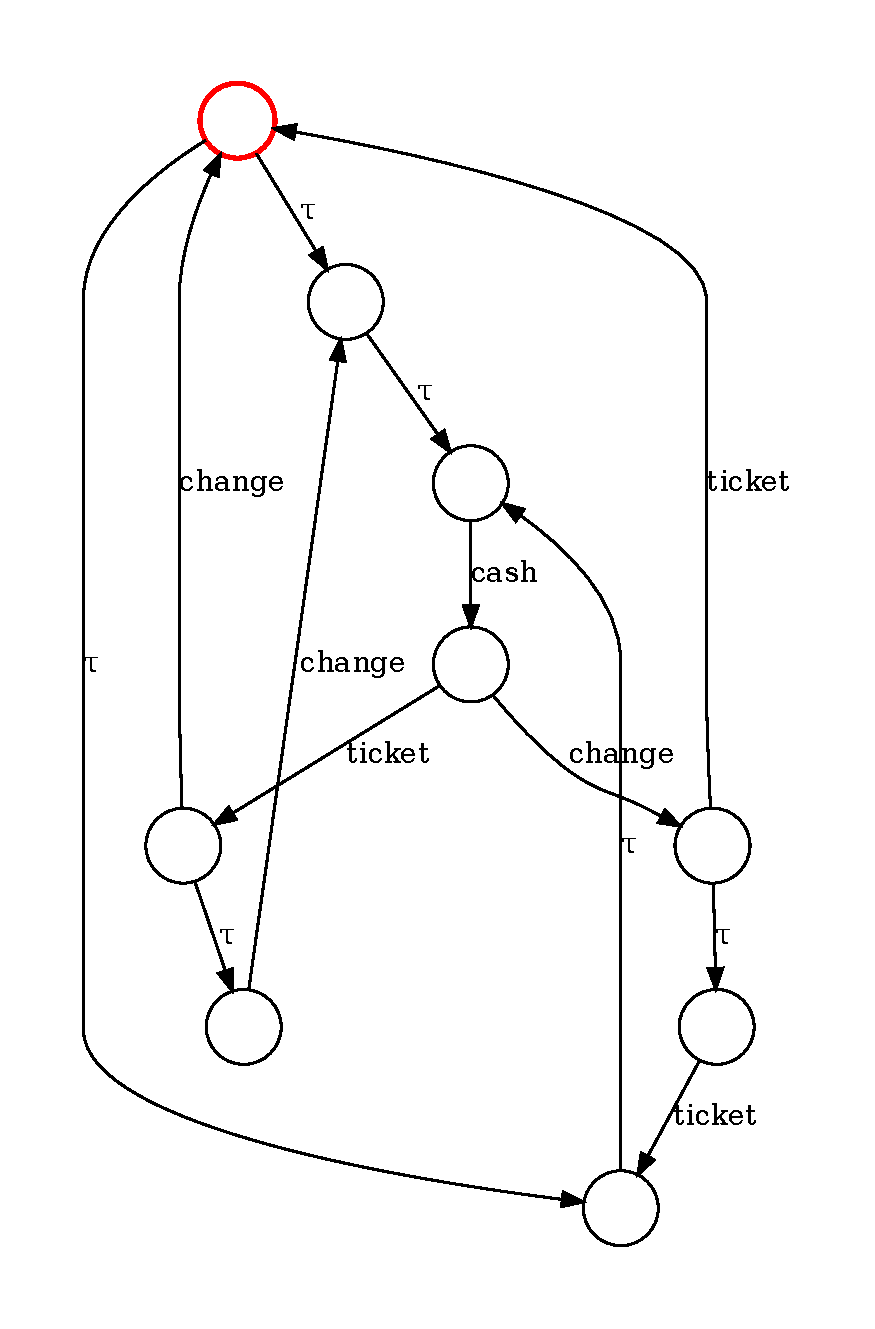
\includegraphics[scale=0.55]{images/parking_permit_mch_lts.pdf}
	\end{center}
\end{figure}

In \CSPcoq, it is also possible to generate such a graph displaying the behaviours (process bodies) associated with each state. Although this decreases the graph readability, it permits the user to know precisely the behaviour represented by each state.

% ---
\section{Traces refinement}
\label{section:traces}
% ---

As we have seen in Section~\ref{subsection:traces-refinement}, a simple but effective way to analyse the behaviour of a process is through the sequence of externally visible events that such a process is capable of performing over time. This communication history is called \emph{trace}. We may perceive a trace as a list of actions that takes from one state to another in an LTS. In Section~\ref{section:traces-concepts} we present our characterisation of traces in Coq, and in Section~\ref{section:quickchick} we explain how we use QuickChick to analyse traces-refinement expressions.

% ---
\subsection{Traces-related concepts}
\label{section:traces-concepts}
% ---

Like the other concepts of CSP we have discussed so far, traces are also formalised in \CSPcoq{}. This concept is defined in terms of a list of events that can be observed by the environment and, thus, $ \tau $ is not considered here. Although our definition of \emph{trace} allows the presence of $\tau$, the way we build traces prevents its appearance.

\begin{coqdoccode}
	\coqdocnoindent
	\coqdockw{Definition} \coqdocvar{trace} := \coqdocvar{list} \coqdocvar{event\_tau\_tick}.\coqdoceol
\end{coqdoccode}

After defining this new type, we can formalise being a trace as a relationship between a process P and a list of events L, so that it is possible to create logical propositions that involve assessing whether L is a trace of P. This relationship encodes the following inference rules:

\begin{itemize}
	\item the empty list is a trace of any process;
	\begin{prooftree}
		\AxiomC{}
		\UnaryInfC{$ \mathit{trace} \ P \ nil $}
	\end{prooftree}

	\item a non-empty list $L = h :: tl$ is a trace of a process $P$ if $P$ behaves as $Q$ after communicating $h$, which cannot be $\tau$, and the remaining events of this list is a trace of the process resulting from this communication;
	\begin{prooftree}
		\AxiomC{$ P \trans[h] Q $}
		\AxiomC{$ \mathit{trace} \ Q \ tl $}
		\RightLabel{\quad ($ h \notin \{\tau\} $)}
		\BinaryInfC{$ \mathit{trace} \ P \ (h :: tl) $}
	\end{prooftree}

	\item similarly, a list $L$ is a trace of a process $P$ if $ \tau $ can be performed by $P$ and $L$ is a trace of the process resulting from this communication.
	\begin{prooftree}
		\AxiomC{$ P \trans[\tau] Q $}
		\AxiomC{$ \mathit{trace} \ Q \ L $}
		\BinaryInfC{$ \mathit{trace} \ P \ L $}
	\end{prooftree}
\end{itemize}

To illustrate this concept, consider once again the process MACHINE, whose LTS is represented by the graph in Figure~\ref{image:machine_lts}. Examining this figure, one can note that the sequence of events <cash, ticket, change> is a trace of this process. First, the process communicates the internal event $ \tau $ twice, in order to unfold both sides of the parallel combination. Then, it proceeds to communicate the event cash, as the joint step of the MACHINE components (processes TICKET and CHANGE). Finally, the left-hand side of the parallel composition may communicate first, performing the event ticket; followed by event change, communicated by the right-hand side of the parallel composition. Remember that a trace consists of visible events only (also considering $\tick$), therefore the first two communicated events, which both happen to be $ \tau $, do not appear in the trace.

Now, we create an inductively defined proposition to formalise the traces notion, encoding the aforementioned rules, which are translated to three constructors of \coqdocvar{traceR'}. The propositional function \coqdocvar{traceR} is responsible for retrieving the process body associated with the provided process name.

\begin{coqdoccode}
	\coqdocnoindent
	\coqdockw{Inductive} \coqdocvar{traceR'} : \coqdocvar{specification} \ensuremath{\rightarrow} \coqdocvar{proc\_body} \ensuremath{\rightarrow} \coqdocvar{trace} \ensuremath{\rightarrow} \coqdockw{Prop} :=\coqdoceol
	\coqdocindent{1.00em}
	\ensuremath{|} \coqdocvar{empty\_trace\_rule} (\coqdocvar{S} : \coqdocvar{specification}) (\coqdocvar{P} : \coqdocvar{proc\_body}) :\coqdoceol
	\coqdocindent{2.00em}
	\coqdocvar{traceR'} \coqdocvar{S} \coqdocvar{P} \coqdocvar{nil}\coqdoceol
	\coqdocindent{1.00em}
	\ensuremath{|} \coqdocvar{event\_trace\_rule} (\coqdocvar{S} : \coqdocvar{specification}) (\coqdocvar{P} \coqdocvar{P'} : \coqdocvar{proc\_body}) (\coqdocvar{h} : \coqdocvar{event\_tau\_tick}) (\coqdocvar{tl} : \coqdocvar{trace}) :\coqdoceol
	\coqdocindent{2.00em}
	\ensuremath{\lnot} \coqdocvar{eq} \coqdocvar{h} \coqdocvar{Tau} \ensuremath{\rightarrow}\coqdoceol
	\coqdocindent{2.00em}
	(\coqdocvar{S} \# \coqdocvar{P} // \coqdocvar{h} ==> \coqdocvar{P'}) \ensuremath{\rightarrow}\coqdoceol
	\coqdocindent{2.00em}
	\coqdocvar{traceR'} \coqdocvar{S} \coqdocvar{P'} \coqdocvar{tl} \ensuremath{\rightarrow}\coqdoceol
	\coqdocindent{2.00em}
	\coqdocvar{traceR'} \coqdocvar{S} \coqdocvar{P} (\coqdocvar{h}::\coqdocvar{tl})\coqdoceol
	\coqdocindent{1.00em}
	\ensuremath{|} \coqdocvar{tau\_trace\_rule} (\coqdocvar{S} : \coqdocvar{specification}) (\coqdocvar{P} \coqdocvar{P'} : \coqdocvar{proc\_body}) (\coqdocvar{t} : \coqdocvar{trace}) :\coqdoceol
	\coqdocindent{2.00em}
	(\coqdocvar{S} \# \coqdocvar{P} // \coqdocvar{Tau} ==> \coqdocvar{P'}) \ensuremath{\rightarrow}\coqdoceol
	\coqdocindent{2.00em}
	\coqdocvar{traceR'} \coqdocvar{S} \coqdocvar{P'} \coqdocvar{t} \ensuremath{\rightarrow}\coqdoceol
	\coqdocindent{2.00em}
	\coqdocvar{traceR'} \coqdocvar{S} \coqdocvar{P} \coqdocvar{t}.\coqdoceol
	\coqdocemptyline
	\coqdocnoindent
	\coqdockw{Definition} \coqdocvar{traceR} (\coqdocvar{S} : \coqdocvar{specification}) (\coqdocvar{proc\_name} : \coqdocvar{string}) (\coqdocvar{t} : \coqdocvar{trace}) :=\coqdoceol
	\coqdocindent{1.00em}
	\coqdockw{match} (\coqdocvar{get\_proc\_body} \coqdocvar{S} \coqdocvar{proc\_name}) \coqdockw{with}\coqdoceol
	\coqdocindent{1.00em}
	\ensuremath{|} \coqdocvar{Some} \coqdocvar{body} \ensuremath{\Rightarrow} \coqdocvar{traceR'} \coqdocvar{S} \coqdocvar{body} \coqdocvar{t}\coqdoceol
	\coqdocindent{1.00em}
	\ensuremath{|} \coqdocvar{None} \ensuremath{\Rightarrow} \coqdocvar{False}\coqdoceol
	\coqdocindent{1.00em}
	\coqdockw{end}.\coqdoceol
\end{coqdoccode}

Note that the inference rules described before, in the order they were presented, correspond, respectively, to the constructors \coqdocvar{empty\_trace\_rule,} \coqdocvar{event\_trace\_rule}, and \coqdocvar{tau\_trace\_rule} of the \coqdocvar{traceR'} inductive definition.

This definition of traces as a relation allows us not only to make assertions like \emph{traceR S ``P'' L}, given a specification $ S $, a process $ P $ and a list of events $ L $, but also prove them in Coq by applying the constructors from the inductive declarations of traces and SOS.

It turns out that, the proof that $L$ is a trace of $P$ grows proportionally to the size of the list (trace). Additionally, these proofs also become quite repetitive. Fortunately, this repetition allows us to define an algorithm (decision procedure) to automatically prove assertions of this kind. Therefore, we have created a tactic macro for this purpose.

This algorithm can be defined as follows. If the goal is to prove the trace relation for an empty list, apply the rule \coqdocvar{empty\_trace\_rule} and finish the proof. Otherwise, try to make progress by applying each of the other two constructors of \coqdocvar{traceR'}, and then repeating this procedure until the proof is finished. For goals that involve expressions in terms of the \CSPcoq{} semantics (SOS), based o pattern matching, try to make progress using the SOS constructors applicable for the current SOS operator, making once again a recursive call at the end of this step.

The definition \coqdocvar{solve\_trace'}, partially presented in what follows, uses the Ltac language to describe this algorithm as a tactic macro that automatically proves statements of the kind \emph{traceR S ``P'' L}. Note that the first case deals with the situation when the list is empty (\emph{nil}). The second case tries to make progress by applying the \coqdocvar{tau\_trace\_rule} and \coqdocvar{event\_trace\_rule} constructors. Then, we have many cases considering the application of SOS constructors. In the end, we have some additional cases for proving some specific propositions, involving \coqdocvar{set\_In} and disjunctions. Finally, the tactic \coqdocvar{solve\_trace} works unfolding the definition \emph{traceR}, performing simplification and, then, invoking the tactic \coqdocvar{solve\_trace'}.

\begin{coqdoccode}
	\coqdocnoindent
	\coqdockw{Ltac} \coqdocvar{solve\_trace'} :=\coqdoceol
	\coqdocindent{1.00em}
	\coqdocvar{multimatch} \coqdockw{goal} \coqdockw{with}\coqdoceol
	\coqdocindent{1.00em}
	\ensuremath{|} \ensuremath{\vdash} \coqdocvar{traceR'} \coqdocvar{\_} \coqdocvar{\_} \coqdocvar{nil} \ensuremath{\Rightarrow} \coqdoctac{apply} \coqdocvar{empty\_trace\_rule}\coqdoceol
	\coqdocindent{1.00em}
	\ensuremath{|} \ensuremath{\vdash} \coqdocvar{traceR'} \coqdocvar{\_} \coqdocvar{\_} \coqdocvar{\_} \ensuremath{\Rightarrow}\coqdoceol
	\coqdocindent{2.00em}
	(\coqdoctac{eapply} \coqdocvar{tau\_trace\_rule}\coqdoceol
	\coqdocindent{2.00em}
	+ \coqdoctac{eapply} \coqdocvar{event\_trace\_rule}); \coqdocvar{solve\_trace'}\coqdoceol
	\coqdocindent{1.00em}
	\ensuremath{|} \ensuremath{\vdash} \coqdocvar{\_} \# \coqdocvar{\_} --> \coqdocvar{\_} // \coqdocvar{\_} ==> \coqdocvar{\_} \ensuremath{\Rightarrow} \coqdoctac{apply} \coqdocvar{prefix\_rule}\coqdoceol
	\coqdocindent{1.00em}
	\ensuremath{|} \ensuremath{\vdash} \coqdocvar{\_} \# \coqdocvar{ProcRef} \coqdocvar{\_} // \coqdocvar{\_} ==> \coqdocvar{\_} \ensuremath{\Rightarrow} \coqdoctac{eapply} \coqdocvar{reference\_rule}; \coqdocvar{solve\_trace'}\coqdoceol
	\coqdocindent{1.00em}
	\ensuremath{|} \ensuremath{\vdash} \coqdocvar{\_} \# \coqdocvar{\_} [] \coqdocvar{\_} // \coqdocvar{\_} ==> \coqdocvar{\_} \ensuremath{\Rightarrow}\coqdoceol
	\coqdocindent{2.00em}
	(\coqdoctac{eapply} \coqdocvar{ext\_choice\_tau\_left\_rule}\coqdoceol
	\coqdocindent{2.00em}
	+ \coqdoctac{eapply} \coqdocvar{ext\_choice\_tau\_right\_rule}\coqdoceol
	\coqdocindent{2.00em}
	+ \coqdoctac{eapply} \coqdocvar{ext\_choice\_left\_rule}\coqdoceol
	\coqdocindent{2.00em}
	+ \coqdoctac{eapply} \coqdocvar{ext\_choice\_right\_rule}); \coqdocvar{solve\_trace'}\coqdoceol
	\coqdocindent{1.00em}
	$\vdots$\coqdoceol
	\coqdocindent{1.00em}
	\ensuremath{|} \ensuremath{\vdash} \coqdocvar{\_} \ensuremath{\not=} \coqdocvar{\_} \ensuremath{\Rightarrow} \coqdoctac{unfold} \coqdocvar{not}; \coqdockw{let} \coqdocvar{H} := \coqdoctac{fresh} ``H'' \coqdoctac{in} (\coqdoctac{intros} \coqdocvar{H}; \coqdoctac{inversion} \coqdocvar{H})\coqdoceol
	\coqdocindent{1.00em}
	\ensuremath{|} \ensuremath{\vdash} \coqdocvar{\_} = \coqdocvar{\_} \ensuremath{\Rightarrow} \coqdoctac{reflexivity}\coqdoceol
	\coqdocindent{1.00em}
	\ensuremath{|} \ensuremath{\vdash} \coqdocvar{set\_In} \coqdocvar{\_} \coqdocvar{\_} \ensuremath{\Rightarrow} \coqdoctac{simpl}; \coqdocvar{solve\_trace'}\coqdoceol
	\coqdocindent{1.00em}
	\ensuremath{|} \ensuremath{\vdash} \ensuremath{\lnot} \coqdocvar{set\_In} \coqdocvar{\_} \coqdocvar{\_} \ensuremath{\Rightarrow} \coqdocvar{solve\_not\_in}\coqdoceol
	\coqdocindent{1.00em}
	\ensuremath{|} \ensuremath{\vdash} \coqdocvar{\_} \ensuremath{\lor} \coqdocvar{\_} \ensuremath{\Rightarrow} (\coqdoctac{left} + \coqdoctac{right}); \coqdocvar{solve\_trace'}\coqdoceol
	\coqdocindent{1.00em}
	\coqdockw{end}.\coqdoceol
	\coqdocemptyline
	\coqdocnoindent
	\coqdockw{Ltac} \coqdocvar{solve\_trace} := \coqdoctac{unfold} \coqdocvar{traceR}; \coqdoctac{simpl}; \coqdocvar{solve\_trace'}.\coqdoceol
\end{coqdoccode}

The following proof revisits the trace example we have discussed earlier in this section. Using our tactic macro \coqdocvar{solve\_trace}, we can automatically prove that the list of events <cash, ticket, change> is indeed a trace of the process MACHINE (\autoref{image:machine_lts}).

\begin{coqdoccode}
	\coqdocnoindent
	\coqdockw{Example} \coqdocvar{MACHINE\_TRACE} :\coqdoceol
	\coqdocindent{1.00em}
	\coqdocvar{traceR} \coqdocvar{PARKING\_PERMIT\_MCH} ``MACHINE'' [``cash'' ; ``ticket'' ; ``change''].\coqdoceol
	\coqdocnoindent
	\coqdockw{Proof}. \coqdocvar{solve\_trace}. \coqdockw{Qed}.\coqdoceol
\end{coqdoccode}

Provided the definitions we have presented so far, we can finally formulate in Coq the concept of refinement according to the traces model, along with an appropriate notation for this relationship.

\begin{coqdoccode}
	\coqdocnoindent
	\coqdockw{Definition} \coqdocvar{trace\_refinement} (\coqdocvar{S} : \coqdocvar{specification}) (\coqdocvar{Spec} \coqdocvar{Imp} : \coqdocvar{string}) : \coqdockw{Prop} :=\coqdoceol
	\coqdocindent{1.00em}
	\coqdockw{\ensuremath{\forall}} (\coqdocvar{t} : \coqdocvar{trace}), \coqdocvar{traceR} \coqdocvar{S} \coqdocvar{Imp} \coqdocvar{t} \ensuremath{\rightarrow} \coqdocvar{traceR} \coqdocvar{S} \coqdocvar{Spec} \coqdocvar{t}.\coqdoceol
	\coqdocemptyline
	\coqdocnoindent
	\coqdockw{Notation} ``S `\#' P `[T=' Q'' := (\coqdocvar{trace\_refinement} \coqdocvar{S} \coqdocvar{P} \coqdocvar{Q})\coqdoceol
	\coqdocindent{1.00em}
	(\coqdoctac{at} \coqdockw{level} 150, \coqdoctac{left} \coqdockw{associativity}).\coqdoceol
\end{coqdoccode}

As we have explained in Section~\ref{subsection:traces-refinement}, this definition states that an implementation Q refines a specification P, according to the traces model, if, and only if, every trace of Q is also a trace of P.

% ---
\subsection{Checking refinement with QuickChick}
\label{section:quickchick}
% ---

In the context of this work, the QuickChick library was used to random test the refinement property according to the traces model. Our goal is to obtain a simple and automated way to test this property that relates two processes, Imp and Spec, eventually finding counterexamples for the traces refinement relation. In other words, we have developed a checker in QuickChick that tries to find a counterexample of a refinement expression by means of random property-based testing.

In order to create this checker, we first need to define a generator of random inputs, which, in our case, consist of traces for a given process. Thus, we define a random generator that takes a ``specification'' process and an arbitrary natural number to limit the maximum number of events in the trace. This generator returns a trace for the given process, whose size is limited by the third parameter. Proving that this generator is correct (i.e., all traces generated for a process $P$ are indeed traces of $P$ according to definition \coqdocvar{traceR}) remains as a future work.

The function \coqdocvar{gen\_valid\_trace} defines our generator by yielding an instance of the G Monad\footnote{More information available at \url{https://softwarefoundations.cis.upenn.edu/qc-current/QC.html}}. This function, as others presented before, retrieves the process body associated with the provided process identifier. Then, it calls the auxiliary function \coqdocvar{gen\_valid\_trace'}.

\begin{coqdoccode}
	\coqdocnoindent
	\coqdockw{Definition} \coqdocvar{gen\_valid\_trace}\coqdoceol
	\coqdocindent{1.00em}
	(\coqdocvar{S} : \coqdocvar{specification}) (\coqdocvar{proc\_id} : \coqdocvar{string}) (\coqdocvar{size} : \coqdocvar{nat})\coqdoceol
	\coqdocindent{1.00em}
	: \coqdocvar{G} (\coqdocvar{option} \coqdocvar{semantics\_trace.trace}) :=\coqdoceol
	\coqdocindent{1.00em}
	\coqdockw{match} \coqdocvar{get\_proc\_body} \coqdocvar{S} \coqdocvar{proc\_id} \coqdockw{with}\coqdoceol
	\coqdocindent{1.00em}
	\ensuremath{|} \coqdocvar{None} \ensuremath{\Rightarrow} \coqdocvar{ret} \coqdocvar{None}\coqdoceol
	\coqdocindent{1.00em}
	\ensuremath{|} \coqdocvar{Some} \coqdocvar{P} \ensuremath{\Rightarrow} \coqdocvar{gen\_valid\_trace'} \coqdocvar{S} \coqdocvar{P} \coqdocvar{size}\coqdoceol
	\coqdocindent{1.00em}
	\coqdockw{end}.\coqdoceol
\end{coqdoccode}

The function \coqdocvar{gen\_valid\_trace'} operates as follows. While the third parameter is greater than zero, decide -- based on a given frequency -- whether the generation should stop. If it should continue, generate a transition from the current state of the process, decreasing the argument that limits the trace size; call the generator recursively, passing the state reached by the transition generated in the previous step. Finally, return the concatenation of the event from this transition with the result of the recursive call, if the event is not $\tau$. The function \coqdocvar{freq\_} is responsible for making the probabilistic choice. In our case, the option to end the generation before reaching the limit has $ ((1 / (size + 1)) * 100)\% $ chance to happen, while continuing with the generation has the probability of $ ((size / (size + 1)) * 100)\% $.

\begin{coqdoccode}
	\coqdocnoindent
	\coqdockw{Fixpoint} \coqdocvar{gen\_valid\_trace'}\coqdoceol
	\coqdocindent{1.00em}
	(\coqdocvar{S} : \coqdocvar{specification}) (\coqdocvar{P} : \coqdocvar{proc\_body}) (\coqdocvar{size} : \coqdocvar{nat})\coqdoceol
	\coqdocindent{1.00em}
	: \coqdocvar{G} (\coqdocvar{option} \coqdocvar{semantics\_trace.trace}) :=\coqdoceol
	\coqdocindent{1.00em}
	\coqdockw{match} \coqdocvar{size} \coqdockw{with}\coqdoceol
	\coqdocindent{1.00em}
	\ensuremath{|} \coqdocvar{O} \ensuremath{\Rightarrow} \coqdocvar{ret} \coqdocvar{nil}\coqdoceol
	\coqdocindent{1.00em}
	\ensuremath{|} \coqdocvar{S} \coqdocvar{size'} \ensuremath{\Rightarrow}\coqdoceol
	\coqdocindent{2.00em}
	\coqdocvar{freq\_} (\coqdocvar{ret} \coqdocvar{nil}) [\coqdoceol
	\coqdocindent{3.00em}
	(1, \coqdocvar{ret} \coqdocvar{nil}) ;\coqdoceol
	\coqdocindent{3.00em}
	(\coqdocvar{size},\coqdoceol
	\coqdocindent{4.00em}
	\coqdocvar{bind} (\coqdocvar{gen\_valid\_trans} \coqdocvar{S} \coqdocvar{P}) (\coqdoceol
	\coqdocindent{5.00em}
	\coqdockw{fun} \coqdocvar{t} \ensuremath{\Rightarrow} (\coqdoceol
	\coqdocindent{6.00em}
	\coqdockw{match} \coqdocvar{t} \coqdockw{with}\coqdoceol
	\coqdocindent{6.00em}
	\ensuremath{|} \coqdocvar{nil} \ensuremath{\Rightarrow} \coqdocvar{ret} \coqdocvar{nil}\coqdoceol
	\coqdocindent{6.00em}
	\ensuremath{|} (\coqdocvar{Event} \coqdocvar{e}, \coqdocvar{Q}) :: \coqdocvar{\_} \ensuremath{\Rightarrow}\coqdoceol
	\coqdocindent{7.00em}
	\coqdocvar{bind} (\coqdocvar{gen\_valid\_trace'} \coqdocvar{S} \coqdocvar{Q} \coqdocvar{size'}) (\coqdoceol
	\coqdocindent{8.00em}
	\coqdockw{fun} \coqdocvar{ts} \ensuremath{\Rightarrow} \coqdocvar{ret} (\coqdocvar{Event} \coqdocvar{e} :: \coqdocvar{ts})\coqdoceol
	\coqdocindent{7.00em}
	)\coqdoceol
	\coqdocindent{6.00em}
	\ensuremath{|} (\coqdocvar{Tick}, \coqdocvar{Q}) :: \coqdocvar{\_} \ensuremath{\Rightarrow}\coqdoceol
	\coqdocindent{7.00em}
	\coqdocvar{bind} (\coqdocvar{gen\_valid\_trace'} \coqdocvar{S} \coqdocvar{Q} \coqdocvar{size'}) (\coqdoceol
	\coqdocindent{8.00em}
	\coqdockw{fun} \coqdocvar{ts} \ensuremath{\Rightarrow} \coqdocvar{ret} (\coqdocvar{Tick} :: \coqdocvar{ts})\coqdoceol
	\coqdocindent{7.00em}
	)\coqdoceol
	\coqdocindent{6.00em}
	\ensuremath{|} (\coqdocvar{Tau}, \coqdocvar{Q}) :: \coqdocvar{\_} \ensuremath{\Rightarrow}\coqdoceol
	\coqdocindent{7.00em}
	\coqdocvar{bind} (\coqdocvar{gen\_valid\_trace'} \coqdocvar{S} \coqdocvar{Q} \coqdocvar{size'}) (\coqdoceol
	\coqdocindent{8.00em}
	\coqdockw{fun} \coqdocvar{ts} \ensuremath{\Rightarrow} \coqdocvar{ret} \coqdocvar{ts}\coqdoceol
	\coqdocindent{7.00em}
	)\coqdoceol
	\coqdocindent{6.00em}
	\coqdockw{end}\coqdoceol
	\coqdocindent{5.00em}
	)\coqdoceol
	\coqdocindent{4.00em}
	)\coqdoceol
	\coqdocindent{3.00em}
	)\coqdoceol
	\coqdocindent{2.00em}
	]\coqdoceol
	\coqdocindent{1.00em}
	\coqdockw{end}.\coqdoceol
\end{coqdoccode}

The command that samples traces according to this generator, as well as part of the output of this sampling process are exemplified below.

\begin{coqdoccode}
	\coqdocnoindent
	\coqdocvar{Sample} (\coqdocvar{gen\_valid\_trace} \coqdocvar{PARKING\_PERMIT\_MCH} ``MACHINE'' 10).\coqdoceol
\end{coqdoccode}

\begin{tabbing}
	\emph{Output:}\\
	\emph{[Some []; Some [``cash''; ``change''; ``ticket''; ``cash''; ``change''];}\\
	\emph{Some [``cash'']; Some [``cash''; ``ticket''; ``change''; ``cash'']; Some [];}\\
	\emph{Some [``cash''; ``change''; ``ticket''; ``cash'']; Some [``cash''; ``change''; ``ticket'']; $\dots$]}
\end{tabbing}

As one can see, the definition of \coqdocvar{gen\_valid\_trace'} relies on a generator of random transitions from a given process $P$ (\coqdocvar{gen\_valid\_trans}). The latter generator receives a specification and a process body, and yields a list containing exactly one valid random transition from the given state, where the transition is represented by the pair (action, target\_state). The generation of all emanating transitions from a given process $P$ is performed by \coqdocvar{get\_transitions}, which is a function used in our computable definition of LTSs.

\begin{coqdoccode}
	\coqdocnoindent
	\coqdockw{Definition} \coqdocvar{gen\_valid\_trans}\coqdoceol
	\coqdocindent{1.00em}
	(\coqdocvar{S} : \coqdocvar{specification})\coqdoceol
	\coqdocindent{1.00em}
	(\coqdocvar{P} : \coqdocvar{proc\_body})\coqdoceol
	\coqdocindent{1.00em}
	: \coqdocvar{G} (\coqdocvar{option} (\coqdocvar{list} (\coqdocvar{event\_tau\_tick} \ensuremath{\times} \coqdocvar{proc\_body}))) :=\coqdoceol
	\coqdocindent{1.00em}
	\coqdockw{match} \coqdocvar{get\_transitions} \coqdocvar{S} \coqdocvar{P} \coqdockw{with}\coqdoceol
	\coqdocindent{1.00em}
	\ensuremath{|} \coqdocvar{None} \ensuremath{\Rightarrow} \coqdocvar{ret} \coqdocvar{None}\coqdoceol
	\coqdocindent{1.00em}
	\ensuremath{|} \coqdocvar{Some} \coqdocvar{nil} \ensuremath{\Rightarrow} \coqdocvar{ret} \coqdocvar{nil}\coqdoceol
	\coqdocindent{1.00em}
	\ensuremath{|} \coqdocvar{Some} (\coqdocvar{t} :: \coqdocvar{ts}) \ensuremath{\Rightarrow} \coqdocvar{bind} (\coqdocvar{elems\_} \coqdocvar{t} (\coqdocvar{t} :: \coqdocvar{ts})) (\coqdockw{fun} \coqdocvar{a} \ensuremath{\Rightarrow} \coqdocvar{ret} (\coqdocvar{Some} [\coqdocvar{a}]))\coqdoceol
	\coqdocindent{1.00em}
	\coqdockw{end}.\coqdoceol
\end{coqdoccode}

\noindent The following lines exemplify the usage of \coqdocvar{gen\_valid\_trans}.

\begin{coqdoccode}
	\coqdocnoindent
	\coqdocvar{Sample} (\coqdocvar{gen\_valid\_trans} \coqdocvar{PARKING\_PERMIT\_MCH}\coqdoceol
	\coqdocindent{1.00em}
	(\coqdocvar{ProcRef} ``TICKET''\coqdoceol
	\coqdocindent{1.40em} [[ \{\{``cash'', ``ticket''\}\} \symbol{92}\symbol{92} \{\{``cash'', ``change''\}\} ]]\coqdoceol
	\coqdocindent{1.40em}\coqdocvar{ProcRef} ``CHANGE'')).\coqdoceol
\end{coqdoccode}

\begin{tabbing}
	\emph{Output:}\\
	\emph{[Some [($ \tau $,TICKET [{ticket, cash} || {change, cash}] cash $ \rightarrow $ change $ \rightarrow $ CHANGE)];}\\
	\emph{Some [($ \tau $,cash $ \rightarrow $ ticket $ \rightarrow $ TICKET [{ticket, cash} || {change, cash}] CHANGE)]; $\dots$]}
\end{tabbing}

Note that, since this generator also computes transitions in which $ \tau $ may appear as actions, it is necessary to hide them, so that the generated trace does not consider these internal events. The generator \coqdocvar{gen\_valid\_trace} does so by concatenating only external events and $\tick$ to the list that will be returned.

Once the random generator of traces is defined, we need an executable property that uses the generated traces to assess a refinement expression. Therefore, we define the function \coqdocvar{check\_trace'} to check whether the trace generated from a process \emph{Imp} is also a trace of a process \emph{Spec}. The idea behind this function is to try to make progress within the given process, one step at a time, consuming the events of the trace in the order in which they appear, while trying to guess non-deterministically when it is necessary to insert a $ \tau $ for the sequence of events to be accepted by the process.

The function \coqdocvar{check\_trace'} initially computes all possible immediate transitions from one state. Then, it filters, from these transitions, those whose action corresponds either to the current element in the list of events (trace), or the internal event. Then, we try to make progress with each of these valid events, performing a recursive call considering each target state obtained from the transitions in the previous step, but removing the corresponding event from the list when applicable -- that is, except $ \tau $. If any of the recursive calls reach an empty list (trace), then the provided trace is indeed a trace of the process. Differently, if none of the recursive calls is able to make progress, then we can assume that this list is not a trace of the process.

\begin{coqdoccode}
	\coqdocnoindent
	\coqdockw{Fixpoint} \coqdocvar{check\_trace'}\coqdoceol
	\coqdocindent{1.00em}
	(\coqdocvar{S} : \coqdocvar{specification})	(\coqdocvar{P} : \coqdocvar{proc\_body})	(\coqdocvar{event\_list} : \coqdocvar{trace}) (\coqdocvar{fuel} : \coqdocvar{nat}) : \coqdocvar{option} \coqdocvar{bool} :=\coqdoceol
	\coqdocindent{1.00em}
	\coqdockw{match} \coqdocvar{fuel}, \coqdocvar{event\_list} \coqdockw{with}\coqdoceol
	\coqdocindent{1.00em}
	\ensuremath{|} \coqdocvar{\_}, \coqdocvar{nil} \ensuremath{\Rightarrow} \coqdocvar{Some} \coqdocvar{true}\coqdoceol
	\coqdocindent{1.00em}
	\ensuremath{|} \coqdocvar{O}, \coqdocvar{\_} \ensuremath{\Rightarrow} \coqdocvar{None} \coqdoceol
	\coqdocindent{1.00em}
	\ensuremath{|} \coqdocvar{S} \coqdocvar{fuel'}, \coqdocvar{e} :: \coqdocvar{es} \ensuremath{\Rightarrow}\coqdoceol
	\coqdocindent{2.00em}
	\coqdockw{match} \coqdocvar{get\_transitions} \coqdocvar{S} \coqdocvar{P} \coqdockw{with}\coqdoceol
	\coqdocindent{2.00em}
	\ensuremath{|} \coqdocvar{None} \ensuremath{\Rightarrow} \coqdocvar{None}\coqdoceol
	\coqdocindent{2.00em}
	\ensuremath{|} \coqdocvar{Some} \coqdocvar{t} \ensuremath{\Rightarrow}\coqdoceol
	\coqdocindent{3.00em}
	\coqdockw{let} \coqdocvar{available\_moves} := \coqdocvar{t} \coqdoctac{in}\coqdoceol
	\coqdocindent{3.00em}
	\coqdockw{let} \coqdocvar{valid\_moves} := \coqdocvar{filter} (\coqdoceol
	\coqdocindent{4.00em}
	\coqdockw{fun} \coqdocvar{t} \ensuremath{\Rightarrow} (\coqdocvar{is\_equal} (\coqdocvar{fst} \coqdocvar{t}) (\coqdocvar{Event} \coqdocvar{e}))\coqdoceol
	\coqdocindent{5.00em}
	|| (\coqdocvar{is\_equal} (\coqdocvar{fst} \coqdocvar{t}) \coqdocvar{Tau})\coqdoceol
	\coqdocindent{5.00em}
	|| (\coqdocvar{is\_equal} (\coqdocvar{fst} \coqdocvar{t}) \coqdocvar{Tick})\coqdoceol
	\coqdocindent{3.00em}
	) \coqdocvar{available\_moves} \coqdoctac{in}\coqdoceol
	\coqdocindent{3.00em}
	\coqdockw{match} \coqdocvar{valid\_moves} \coqdockw{with}\coqdoceol
	\coqdocindent{3.00em}
	\ensuremath{|} \coqdocvar{nil} \ensuremath{\Rightarrow} \coqdocvar{Some} \coqdocvar{false}\coqdoceol
	\coqdocindent{3.00em}
	\ensuremath{|} \coqdocvar{\_} \ensuremath{\Rightarrow}\coqdoceol
	\coqdocindent{4.00em}
	\coqdockw{let} \coqdocvar{result} := \coqdocvar{map} (\coqdockw{fun} \coqdocvar{t} \ensuremath{\Rightarrow}\coqdoceol
	\coqdocindent{5.00em}
	\coqdockw{if} \coqdocvar{negb} (\coqdocvar{is\_equal} (\coqdocvar{fst} \coqdocvar{t}) (\coqdocvar{Tau}))\coqdoceol
	\coqdocindent{5.00em}
	\coqdockw{then} \coqdocvar{check\_trace'} \coqdocvar{S} (\coqdocvar{snd} \coqdocvar{t}) \coqdocvar{es} \coqdocvar{fuel'}\coqdoceol
	\coqdocindent{5.00em}
	\coqdockw{else} \coqdocvar{check\_trace'} \coqdocvar{S} (\coqdocvar{snd} \coqdocvar{t}) (\coqdocvar{e} :: \coqdocvar{es}) \coqdocvar{fuel'}\coqdoceol
	\coqdocindent{4.00em}
	) \coqdocvar{valid\_moves} \coqdoctac{in}\coqdoceol
	\coqdocindent{4.00em}
	\coqdockw{if} \coqdocvar{existsb} (\coqdockw{fun} \coqdocvar{o} \ensuremath{\Rightarrow}\coqdoceol
	\coqdocindent{5.00em}
	\coqdockw{match} \coqdocvar{o} \coqdockw{with}\coqdoceol
	\coqdocindent{5.00em}
	\ensuremath{|} \coqdocvar{Some} \coqdocvar{true} \ensuremath{\Rightarrow} \coqdocvar{true}\coqdoceol
	\coqdocindent{5.00em}
	\ensuremath{|} \coqdocvar{\_} \ensuremath{\Rightarrow} \coqdocvar{false}\coqdoceol
	\coqdocindent{5.00em}
	\coqdockw{end}) \coqdocvar{result}\coqdoceol
	\coqdocindent{4.00em}
	\coqdockw{then} \coqdocvar{Some} \coqdocvar{true}\coqdoceol
	\coqdocindent{4.00em}
	\coqdockw{else} \coqdockw{if} \coqdocvar{forallb} (\coqdockw{fun} \coqdocvar{o} \ensuremath{\Rightarrow}\coqdoceol
	\coqdocindent{5.00em}
	\coqdockw{match} \coqdocvar{o} \coqdockw{with}\coqdoceol
	\coqdocindent{5.00em}
	\ensuremath{|} \coqdocvar{Some} \coqdocvar{false} \ensuremath{\Rightarrow} \coqdocvar{true}\coqdoceol
	\coqdocindent{5.00em}
	\ensuremath{|} \coqdocvar{\_} \ensuremath{\Rightarrow} \coqdocvar{false}\coqdoceol
	\coqdocindent{5.00em}
	\coqdockw{end}) \coqdocvar{result}\coqdoceol
	\coqdocindent{4.00em}
	\coqdockw{then} \coqdocvar{Some} \coqdocvar{false}\coqdoceol
	\coqdocindent{4.00em}
	\coqdockw{else} \coqdocvar{None}\coqdoceol
	\coqdocindent{3.00em}
	\coqdockw{end}\coqdoceol
	\coqdocindent{2.00em}
	\coqdockw{end}\coqdoceol
	\coqdocindent{1.00em}
	\coqdockw{end}.\coqdoceol
\end{coqdoccode}

The function \coqdocvar{check\_trace'} is called by \coqdocvar{check\_trace}, which retrieves the process body associated with the provided process identifier.

\begin{coqdoccode}
	\coqdocemptyline
	\coqdocnoindent
	\coqdockw{Definition} \coqdocvar{check\_trace}\coqdoceol
	\coqdocindent{1.00em}
	(\coqdocvar{S} : \coqdocvar{specification}) (\coqdocvar{proc\_id} : \coqdocvar{string}) (\coqdocvar{event\_list} : \coqdocvar{trace}) 	(\coqdocvar{fuel} : \coqdocvar{nat}) : \coqdocvar{option} \coqdocvar{bool} :=\coqdoceol
	\coqdocindent{1.00em}
	\coqdockw{match} \coqdocvar{fuel}, \coqdocvar{get\_proc\_body} \coqdocvar{S} \coqdocvar{proc\_id} \coqdockw{with}\coqdoceol
	\coqdocindent{1.00em}
	\ensuremath{|} \coqdocvar{O}, \coqdocvar{\_} \ensuremath{|} \coqdocvar{\_}, \coqdocvar{None} \ensuremath{\Rightarrow} \coqdocvar{None}\coqdoceol
	\coqdocindent{1.00em}
	\ensuremath{|} \coqdocvar{S} \coqdocvar{fuel'}, \coqdocvar{Some} \coqdocvar{P} \ensuremath{\Rightarrow} \coqdocvar{check\_trace'} \coqdocvar{S} \coqdocvar{P} \coqdocvar{event\_list} \coqdocvar{fuel'}\coqdoceol
	\coqdocindent{1.00em}
	\coqdockw{end}.\coqdoceol
\end{coqdoccode}

Finally, the function \coqdocvar{traceP} provides the given trace to \coqdocvar{check\_trace} and propagates the boolean yielded by the latter function.

\begin{coqdoccode}
	\coqdocnoindent
	\coqdockw{Definition} \coqdocvar{traceP}\coqdoceol
	\coqdocindent{1.00em}
	(\coqdocvar{S} : \coqdocvar{specification})
	(\coqdocvar{proc\_id} : \coqdocvar{string})
	(\coqdocvar{fuel} : \coqdocvar{nat})\coqdoceol
	\coqdocindent{1.00em}
	(\coqdocvar{t} : \coqdocvar{option} \coqdocvar{semantics\_trace.trace}) : \coqdocvar{bool} :=\coqdoceol
	\coqdocindent{1.00em}
	\coqdockw{match} \coqdocvar{t} \coqdockw{with}\coqdoceol
	\coqdocindent{1.00em}
	\ensuremath{|} \coqdocvar{None} \ensuremath{\Rightarrow} \coqdocvar{false}\coqdoceol
	\coqdocindent{1.00em}
	\ensuremath{|} \coqdocvar{Some} \coqdocvar{t'} \ensuremath{\Rightarrow}\coqdoceol
	\coqdocindent{2.00em}
	\coqdockw{match} \coqdocvar{check\_trace} \coqdocvar{S} \coqdocvar{proc\_id} \coqdocvar{t'} \coqdocvar{fuel} \coqdockw{with}\coqdoceol
	\coqdocindent{2.00em}
	\ensuremath{|} \coqdocvar{None} \ensuremath{\Rightarrow} \coqdocvar{false}\coqdoceol
	\coqdocindent{2.00em}
	\ensuremath{|} \coqdocvar{Some} \coqdocvar{b} \ensuremath{\Rightarrow} \coqdocvar{b}\coqdoceol
	\coqdocindent{2.00em}
	\coqdockw{end}\coqdoceol
	\coqdocindent{1.00em}
	\coqdockw{end}.\coqdoceol
\end{coqdoccode}

Provided these definitions, we define the refinement-property checker. This checker tests whether every randomly generated trace of an implementation process is also a trace of a specification process. This definition reflects the formal definition of the trace-refinement relation presented in Section~\ref{section:traces-concepts}.

\begin{coqdoccode}
	\coqdocnoindent
	\coqdockw{Definition} \coqdocvar{trace\_refinement\_checker}\coqdoceol
	\coqdocindent{1.00em}
	(\coqdocvar{S} : \coqdocvar{specification})
	(\coqdocvar{Imp} \coqdocvar{Spec} : \coqdocvar{string})
	(\coqdocvar{trace\_max\_size} : \coqdocvar{nat})
	(\coqdocvar{fuel} : \coqdocvar{nat}) : \coqdocvar{Checker} :=\coqdoceol
	\coqdocindent{2.00em}
	\coqdocvar{forAll} (\coqdocvar{gen\_valid\_trace} \coqdocvar{S} \coqdocvar{Imp} \coqdocvar{trace\_max\_size}) (\coqdocvar{traceP} \coqdocvar{S} \coqdocvar{Spec} \coqdocvar{fuel}).\coqdoceol
\end{coqdoccode}

To illustrate the verification of this executable property, consider the following \CSPcoq{} specification.

\begin{coqdoccode}
	\coqdocnoindent
	\coqdockw{Definition} \coqdocvar{EXAMPLE} : \coqdocvar{specification}.\coqdoceol
	\coqdocnoindent
	\coqdockw{Proof}.\coqdoceol
	\coqdocindent{1.00em}
	\coqdocvar{solve\_spec\_ctx\_rules} (\coqdoceol
	\coqdocindent{2.00em}
	\coqdocvar{Build\_Spec}\coqdoceol
	\coqdocindent{3.00em}
	[ \coqdocvar{Channel} \{\{``a'', ``b'', ``c''\}\} ]\coqdoceol
	\coqdocindent{3.00em}
	[ ``P'' ::= ``a'' -{}-> ``b'' -{}-> \coqdocvar{ProcRef} ``P'' ;\coqdoceol
	\coqdocindent{4.00em}
	``Q'' ::= (``a'' -{}-> ``b'' -{}-> \coqdocvar{ProcRef} ``Q'') [] (``c'' -{}-> \coqdocvar{STOP}) ]\coqdoceol
	\coqdocindent{1.00em}
	).\coqdoceol
	\coqdocnoindent
	\coqdockw{Defined}.\coqdoceol
\end{coqdoccode}

If we may want to check whether ``Q'' trace-refines ``P'', that is, if every trace of ``Q'' is also a trace of ``P'', we invoke our checker with the command \coqdocvar{QuickChick}, passing, for instance, 5 as the maximum trace size and the arbitrary integer 1000 as the fuel argument (to limit the number of performed recursions).

\begin{coqdoccode}
	\coqdocnoindent
	\coqdocvar{QuickChick} (\coqdocvar{trace\_refinement\_checker} \coqdocvar{EXAMPLE} ``Q'' ``P'' 5 1000).\coqdoceol
\end{coqdoccode}

\begin{tabbing}
	\emph{Some [``c'']} \\
	\emph{*** Failed after 3 tests and 0 shrinks. (0 discards)}
\end{tabbing}

As we are told by the message above, QuickChick performed 3 tests before running into a trace that violates the refinement relation, showing evidence that ``Q'' does not trace-refine ``P'', since [``c''] is a trace of ``Q'', but it is not a trace of ``P''. Differently, note that the process ``Q'' is actually refined by ``P'' (i.e. ``P'' trace-refines ``Q''). We will not be able to prove that statement with our checker though. Instead, it may only lead us to believe that the relation holds, since QuickChick is not able to provide us with any counterexample after executing 10000 tests.

\begin{coqdoccode}
	\coqdocnoindent
	\coqdocvar{QuickChick} (\coqdocvar{trace\_refinement\_checker} \coqdocvar{EXAMPLE} ``P'' ``Q'' 5 1000).\coqdoceol
\end{coqdoccode}

\begin{tabbing}
	\emph{+++ Passed 10000 tests (0 discards)}
\end{tabbing}

Therefore, since this method is, ultimately, a testing solution, we are only interested in counterexamples, which actually show evidence that the refinement relation does not hold between two processes. Passing tests must be considered nothing but a mere indication of a possibly valid refinement expression. In other words, this refinement-checking approach is sound (if the checked property does not hold, the trace-refinement relation does not hold), but it is not complete (if the checked property holds, we can not guarantee whether the trace-refinement relation holds).